% Created 2021-04-15 Thu 13:52
% Intended LaTeX compiler: pdflatex

  \documentclass[oneside]{book}
  \usepackage[T1, T2A]{fontenc}
\usepackage[lutf8]{luainputenc}
\usepackage[english, russian]{babel}
\usepackage{minted}
\usepackage{graphicx}
\usepackage{longtable}
\usepackage{hyperref}
\usepackage{xcolor}
\usepackage{natbib}
\usepackage{amssymb}
\usepackage{stmaryrd}
\usepackage{amsmath}
\usepackage{caption}
\usepackage{mathtools}
\usepackage{amsthm}
\usepackage{tikz}
\usepackage{grffile}
\usepackage{extarrows}
\usepackage{wrapfig}
\usepackage{algorithm}
\usepackage{algorithmic}
\usepackage{lipsum}
\usepackage{rotating}
\usepackage{placeins}
\usepackage[normalem]{ulem}
\usepackage{amsmath}
\usepackage{textcomp}
\usepackage{capt-of}
  
  \addto\captionsrussian{\renewcommand{\chaptername}{Лекция}}
   \usepackage{hyperref}
 \hypersetup{
     colorlinks=true,
     linkcolor=blue,
     filecolor=orange,
     citecolor=black,      
     urlcolor=cyan,
     }

\usetikzlibrary{decorations.markings}
\usetikzlibrary{cd}
\usetikzlibrary{patterns}
\usetikzlibrary{automata, arrows}

\newcommand\addtag{\refstepcounter{equation}\tag{\theequation}}
\newcommand{\eqrefoffset}[1]{\addtocounter{equation}{-#1}(\arabic{equation}\addtocounter{equation}{#1})}
\newcommand{\llb}{\llbracket}
\newcommand{\rrb}{\rrbracket}


\newcommand{\R}{\mathbb{R}}
\renewcommand{\C}{\mathbb{C}}
\newcommand{\N}{\mathbb{N}}
\newcommand{\A}{\mathfrak{A}}
\newcommand{\B}{\mathfrak{B}}
\newcommand{\rank}{\mathop{\rm rank}\nolimits}
\newcommand{\const}{\var{const}}
\newcommand{\grad}{\mathop{\rm grad}\nolimits}

\newcommand{\todo}{{\color{red}\fbox{\text{Доделать}}}}
\newcommand{\fixme}{{\color{red}\fbox{\text{Исправить}}}}

\newcounter{propertycnt}
\setcounter{propertycnt}{1}
\newcommand{\beginproperty}{\setcounter{propertycnt}{1}}

\theoremstyle{plain}
\newtheorem{propertyinner}{Свойство}
\newenvironment{property}{
  \renewcommand\thepropertyinner{\arabic{propertycnt}}
  \propertyinner
}{\endpropertyinner\stepcounter{propertycnt}}
\newtheorem{axiom}{Аксиома}
\newtheorem{lemma}{Лемма}
\newtheorem{manuallemmainner}{Лемма}
\newenvironment{manuallemma}[1]{%
  \renewcommand\themanuallemmainner{#1}%
  \manuallemmainner
}{\endmanuallemmainner}

\theoremstyle{remark}
\newtheorem*{remark}{Примечание}
\newtheorem*{solution}{Решение}
\newtheorem{corollary}{Следствие}[theorem]
\newtheorem*{examp}{Пример}
\newtheorem*{observation}{Наблюдение}

\theoremstyle{definition}
\newtheorem{task}{Задача}
\newtheorem{theorem}{Теорема}[section]
\newtheorem*{definition}{Определение}
\newtheorem*{symb}{Обозначение}
\newtheorem{manualtheoreminner}{Теорема}
\newenvironment{manualtheorem}[1]{%
  \renewcommand\themanualtheoreminner{#1}%
  \manualtheoreminner
}{\endmanualtheoreminner}
\captionsetup{justification=centering,margin=2cm}
\newenvironment{colored}[1]{\color{#1}}{}

\tikzset{->-/.style={decoration={
  markings,
  mark=at position .5 with {\arrow{>}}},postaction={decorate}}}
\makeatletter
\newcommand*{\relrelbarsep}{.386ex}
\newcommand*{\relrelbar}{%
  \mathrel{%
    \mathpalette\@relrelbar\relrelbarsep
  }%
}
\newcommand*{\@relrelbar}[2]{%
  \raise#2\hbox to 0pt{$\m@th#1\relbar$\hss}%
  \lower#2\hbox{$\m@th#1\relbar$}%
}
\providecommand*{\rightrightarrowsfill@}{%
  \arrowfill@\relrelbar\relrelbar\rightrightarrows
}
\providecommand*{\leftleftarrowsfill@}{%
  \arrowfill@\leftleftarrows\relrelbar\relrelbar
}
\providecommand*{\xrightrightarrows}[2][]{%
  \ext@arrow 0359\rightrightarrowsfill@{#1}{#2}%
}
\providecommand*{\xleftleftarrows}[2][]{%
  \ext@arrow 3095\leftleftarrowsfill@{#1}{#2}%
}
\makeatother

\newenvironment{rualgo}[1][]
  {\begin{algorithm}[#1]
     \selectlanguage{russian}%
     \floatname{algorithm}{Алгоритм}%
     \renewcommand{\algorithmicif}{{\color{red}\textbf{если}}}%
     \renewcommand{\algorithmicthen}{{\color{red}\textbf{тогда}}}%
     \renewcommand{\algorithmicelse}{{\color{red}\textbf{иначе}}}%
     \renewcommand{\algorithmicend}{{\color{red}\textbf{конец}}}%
     \renewcommand{\algorithmicfor}{{\color{red}\textbf{для}}}%
     \renewcommand{\algorithmicto}{{\color{red}\textbf{до}}}%
     \renewcommand{\algorithmicdo}{{\color{red}\textbf{делать}}}%
     \renewcommand{\algorithmicwhile}{{\color{red}\textbf{пока}}}%
     \renewcommand{\algorithmicrepeat}{{\color{red}\textbf{повторять}}}%
     \renewcommand{\algorithmicuntil}{{\color{red}\textbf{до тех пор пока}}}%
     \renewcommand{\algorithmicloop}{{\color{red}\textbf{повторять}}}%
     \renewcommand{\algorithmicnot}{{\color{blue}\textbf{не}}}%
     \renewcommand{\algorithmicand}{{\color{blue}\textbf{и}}}%
     \renewcommand{\algorithmicor}{{\color{blue}\textbf{или}}}%
     \renewcommand{\algorithmicrequire}{{\color{blue}\textbf{Ввод}}}%
     \renewcommand{\algorithmicrensure}{{\color{blue}\textbf{Вывод}}}%
     \renewcommand{\algorithmicreturn}{{\color{red}\textbf{Вернуть}}}%
     \renewcommand{\algorithmicrtrue}{{\color{blue}\textbf{истинна}}}%
     \renewcommand{\algorithmicrfalse}{{\color{blue}\textbf{ложь}}}%
     % Set other language requirements
  }
  {\end{algorithm}}
\author{Ilya Yaroshevskiy}
\date{\today}
\title{Лекции по Методам оптимизации 4 семестр}
\hypersetup{
 pdfauthor={Ilya Yaroshevskiy},
 pdftitle={Лекции по Методам оптимизации 4 семестр},
 pdfkeywords={},
 pdfsubject={},
 pdfcreator={Emacs 28.0.50 (Org mode 9.4.4)}, 
 pdflang={English}}
\begin{document}

\maketitle
\tableofcontents


\chapter{}
\label{sec:org22e15d6}
\chapter{Лекции 1 и 2}
\label{sec:org87a464d}
\section{Теория погрешности}
\label{sec:org2558ce6}
\begin{defintion}
Отклонение от теоретического решения
\end{defintion}
Виды погрешности:
\begin{enumerate}
\item Неустранимая погрешность
\begin{examp}
Физические величины, другие константы
\end{examp}
\item Устранимая погрешнеость
Связана с методом решения
\begin{enumerate}
\item Погрешность модели \\
Связана с матиматической формулировкой задачи. Она плохо отображает реальную модель
\item Остаточная погрешность(Погрешноть аппроксимации)
\item Погрешность округления
\item Накапливаемая погрешность \\
Нецелые числа
\end{enumerate}
\end{enumerate}

\noindent\rule{\textwidth}{0.5pt}

\begin{itemize}
\item \(X^*\) --- точное решение \\
\item \(X\) --- Приближенное решение
\item \(X^* - X\) --- погрешность
\item \(\Delta X = |X^* - X|\) --- абсолютная погрешность \\
\(\Delta_X \ge |X^* - X|\) --- предельная абсолютная погрешность, т.е. \[ X - \Delta_X \le X^* \le X + \Delta_X \]
\item \(\delta X = \left|\frac{X^* - X}{|X|}\right|\) --- относительная погрешость \\
\(\delta_X \ge \left|\frac{X^* - X}{|X|}\right|\) --- предельная относительная погрешность
\end{itemize}

\subsection{Значащие цифры}
\label{sec:orge29b75f}
\begin{definition}
Все цифры в изображении отличные от нуля, и нули если они содержатся
между значащими цифрами, или расположены в конце числа и указывают на
сохранение разряды точности.  Нули стоящие левее, отличной от нуля
цифры, не являются значащимицифрами Между ненулевыми, или указывающие
на точность
\end{definition}

\begin{examp}
\(\underbrace{0.00}_\text{незнач.}2080\)
\end{examp}
\begin{examp}
\(689000 = 0.689 \cdot 10^6\) --- 3 значащие цифры
\(689000 = 0.689000 \cdot 10^6\) --- 6 значащих цифр
\end{examp}

\subsection{Верные цифры}
\label{sec:orgb3a390c}
\begin{defintion}
Если, значащая цифра приближенного значения, находящаяся в разряде, в
котором выполняется условие --- абсолютное значение погрешности не
превосходит половину уиницы этого разряда \(\Delta \le 0.5\cdot 10^k\),
где \(k\) --- номер разряда, то она называется верной
\end{defintion}

\begin{examp}
\(a = 3.635\) \\
\(\Delta a = 0.003\) \\
\begin{description}
\item[{(3) \(k = 0\)}] \(\frac{1}{2} \cdot 10^0 = \frac{1}{2} \ge \Delta a\)
\item[{(6) \(k = -1\)}] \(\frac{1}{2} \cdot 10^{-1} = 0.05 \ge \Delta a\)
\item[{(3) \(k = -2\)}] \(\frac{1}{2} \cdot 10^{-2} = 0.005 \ge \Delta a\)
\item[{(5) \(k = -3\)}] \(\frac{1}{2} \cdot 10^{-3} = 0.0005 < \Delta a\) \(\Rightarrow\) 5 --- сомнительная цифра
\end{description}
\end{examp}

\subsection{Распространение погрешности}
\label{sec:org432217d}
\begin{examp}
\(\left(\frac{\sqrt{2} - 1}{\sqrt{2} + 1}\right)^3 = (\sqrt{2} - 1)^6 = (3 - 2\sqrt{2})^3 = 99 - 70\sqrt{2}\) \\
\begin{description}
\item[{\(\sqrt{2}\)}] \[ \frac{7}{5} = 1.4 \]
\[ \frac{17}{12} = 1.41666 \]
\[ \frac{707}{500} = 1.414 \]
\[ \sqrt{2} = 1.4142145624 \]
\end{description}
\end{examp}

\[ \Delta_{x \pm y} = \Delta_x \pm \Delta_y \]
\[ \Delta_{(x\cdot y)} \approx |Y|\Delta_X + |X|\Delta_Y \]
\[ \Delta_{(\frac{x}{y})} \approx \left|\frac{1}{Y}\right|\Delta_X + \left|\frac{X}{Y^2}|\Delta_Y \]
\[ |\Delta u| = |f(x_1 + \Delta x_1, \dots, x_n + \Delta x_n) - f(x_1, \dots, x_n)| \]
\[ |\Delta u| \approx |df(x_1, \dots, x_n)| = \left|\sum_{i=1}^n \frac{\partial u}{\partial x_i}\Delta x_i \right| \le \sum_{i = 1}^n\left|\frac{\partial u}{\partial x_i}\right|\cdot|\Delta x_i| \addtag\label{star_1} \]
\[ |\delta u| = \frac{\ref{star_1}}{|u|} = \sum_{i = 1}^n\left|\frac{\partial u}{\partial x_i}\cdot\frac{1}{u}\right|\cdot|\Delta x_i| = \sum_{i = 1}^n \left|\frac{\partial \ln u}{\partial x_i}\right|\cdot|\Delta x_i| \]
\[ \delta_u = \sum_{i = 1}^n \left|\frac{\partial \ln u}{\partial x_i}\right| \cdot |\Delta x_i| \]
\[ \delta_{(X \pm Y)} = \left|\frac{X}{X \pm Y}\right| \delta_X + \left|\frac{Y}{X \pm Y}\right|\delta_Y \]
\[ \delta_{(X\cdot Y)} = \delta_X + \delta_Y \]
\[ \delta_{(\frac{X}{Y})} = \delta_X + \delta_Y \]

\begin{examp}
\(x = \frac{7}{5}\)
\begin{itemize}
\item \(f_1 = \left(\frac{\sqrt{2} - 1}{\sqrt{2} + 1}\right)\) \\
\[ \delta_{f_1} = 3\left|\frac{1}{x - 1} - \frac{1}{x + 1}\right|\cdot|\Delta X| = 6.25|\Delta X| \]
\item \(f_2 = (\sqrt{2} - 1)^6\) \\
\[ \delta_{f_2} = 6\left|\frac{1}{x - 1}\right|\cdot|\Delta X| = 15|\Delta X| \]
\item \(f_3 = (3 - 2\sqrt{2})^3\)
\[ \delta_{f_3} = 6\left|\frac{1}{3 - 2x}\right|\cdot|\Delta X| = 30|\Delta X| \]
\item \(f_4 = 99 - 70\sqrt{2}\)
\[ \delta_{f_4} = \left|\frac{90}{99 - 70x}\right|\cdot|\Delta X| = 70|\Delta X| \]
\end{itemize}
\end{examp}

\begin{examp}
\[ y^2 - 140y + 1 = 0 \]
Вычислить корни.
\begin{itemize}
\item \(y = 70 - \sqrt{4899}\) \\
\(\sqrt{4899} = 69.992\dots\) \\
\(\sqrt{4899} \approx 69.99\) \\
\(y \approx 70 - 69.99 = 0.01\)
\[ y = \frac{1}{70 + \sqrt{4899}} \]
\(\sqrt{4899} = 69.99;\ 70 + 69.99 = 139.99\) \\
\(y = \frac{1}{140} = 0.00714285 \approx 0.007143\)
\end{itemize}
\end{examp}


\section{Одномерная минимизация функций}
\label{sec:org7ebc51d}
\subsection{Унимодальные функции}
\label{sec:orgf25ade8}
\(f(x) \to \min,\ x \in U\) \\
\(f(x) \to \max \Rightarrow -f(x) \to min\) \\
\(x^* \in U\) --- точка минимума: \(f(x*) \le f(x)\ \forall x \in U\) \\
\(U^*\) --- множество точек минимума \\
\(\tilde{x} \in U: \exists V(\tilde{x})\ \forall x \in V\ f(\tilde{x}) \le f(x)\) --- локальный минимум
\begin{definition}
\(f(x)\) --- \textbf{унимодальная функция} на \([a, b]\), если:
\begin{enumerate}
\item \(f(x)\) --- непрерывна на \([a, b]\)
\item \(\exists \alpha, \beta: a \le \alpha\le\beta\le b\)
\begin{enumerate}
\item Если \(a < \alpha\), то \([a, \alpha]\) \(f(x)\) --- монотонно убывает
\item Если \(\beta < b\), то на \([\beta, b]\) \(f(x)\) --- монотонна возрастает
\item \(\forall x\in[\alpha, \beta]\) \(f(x) = f^* = \min_{[a, b]}f(x)\)
\end{enumerate}
\end{enumerate}
\end{definition}
\begin{remark}
Свойства:
\begin{enumerate}
\item Любая из точек локального минимума является глобальным минимумом на этом же отрезке
\item Функця унимодальная на \([a, b]\)  унимодальна на \([c, d] \subset [a, b]\)
\item \(f(x)\) унимодальна на \([a, b]\) \(a \le x_1 < x_2 \le b\)
\begin{enumerate}
\item если \(f(x_1)\le f(x_2)\), то \(x^* \in [a, x_2]\)
\item если \(f(x_1) > f(x_2)\), то \(x^* \in [x_1, b]\)
\end{enumerate}
\end{enumerate}
\end{remark}
\begin{definition}
\(f(x)\) \textbf{выпукла} на \([a, b]\), если:
\begin{itemize}
\item \(\forall x', x'' \in [a, b]\) и \(\alpha \in [0, 1]\): \\
\[ f(\alpha x' + (1 - \alpha)x'') \le \alpha f(x') + (1 - \alpha)f(x'') \]
\end{itemize}
\end{definition}
\begin{remark}
Свойства:
\begin{enumerate}
\item Если \(f(x)\) на \([a, b]\) \([x', x''] \subset [a, b]\)
\item Всякая выпуклая и непрерывная функция на \([a, b]\) является унимодальной на этом отрезке. Обратное не верно
\end{enumerate}
\end{remark}
\begin{definition}
\(x: f'(x) = 0\) --- \textbf{стационарная точка}
\end{definition}


\subsection{Прямые методы}
\label{sec:org8a1d1ab}
Не требуют вычисление производной. Могут использовать только известные значения. 
\begin{enumerate}
\item Метод дихотомии
\label{sec:orgdebb131}
\[ x_1 = \frac{b + a - \delta}{2}\quad x_2 = \frac{b + a + \delta}{2} \addtag\label{delta_1} \]
\[ \tau = \frac{b - x_1}{b - a} = \frac{x_2 - a}{b - a} \rightarrow \frac{1}{2} \]
\[ X^* [a_i, b_i]\quad \frac{b_i - a_i}{2} \le \varepsilon \]

\begin{enumerate}
\item \(x_1\) и \(x_2\); вычислить \(f(x_1)\) и \(f(x_2)\)
\item \(f(x_1)\) и \(f(x_2)\)
\begin{itemize}
\item Если \(f(x_1) \le f(x_2) \rightarrow [a, x_2]\), т.е. \(b = x_2\)
\item Иначе \([x_1, b] \rightarrow [x_1, b]\), т.е. \(a = x_1\)
\end{itemize}
\item \(\varepsilon_n = \frac{b - a}{2}\) (\(n\) --- номер итерации)
\begin{itemize}
\item Если \(\varepsilon_n > \varepsilon\) --- переход к следующей итерации(шаг 1)
\item Если \(\varepsilon_n \le \varepsilon\), заврешить поиск(шаг 4)
\end{itemize}
\item \(x^* \approx \overline{x} = \frac{a + b}{2} \quad f^* \approx f(\overline{x})\)
\end{enumerate}

\(\ref{delta_1}\quad \delta \in (0, 2\varepsilon)\) \\
Число итерций \(n \ge \log_2\frac{b - a - \delta}{2\varepsilon - \delta}\)
\end{enumerate}
\chapter{}
\label{sec:org5702f9b}
\section{Одномерный поиск}
\label{sec:org410062c}
\subsection{Метод золотого сечения}
\label{sec:org9dc501e}
\begin{remark}
Возьмем отрезок \([0, 1]\)
\begin{itemize}
\item \(x_2 = \tau \Rightarrow x_1 = 1 - \tau\)
\item \(x_1 \Rightarrow x'_2 = 1 - \tau \in [0, \tau]\)
\end{itemize}
\[ \frac{1}{\tau} = \frac{tau}{1 - \tau} \Rightarrow \tau^2 = 1 - \tau\]
\[ \tau = \frac{\sqrt{5} - 1}{2} \approx 0.61803 \]
\begin{itemize}
\item \(x_1 = 1 - \tau = \frac{3 - \sqrt{5}}{2}\)
\item \(x_2 = \tau = \frac{\sqrt{5} - 1}{2}\)
\end{itemize}
\end{remark}
\begin{enumerate}
\item \label{x_1_3} \(x_1 = a + \frac{3 - \sqrt{5}}{2}(b - a)\)
\item \label{x_2_3} \(x_2 = a + \frac{\sqrt{5} - 1}{2}(b - a)\)
\end{enumerate}
\[ \Delta_n = \tau^n(b - a) \]
\[ \varepsilon_n = \frac{\Delta_n}{2} = \frac{1}{2}\left(\frac{\sqrt{5} - 1}{2}\right)^n(b - a) \]
\(\varepsilon\) --- задано. Окончание: \(\varepsilon_n \le \varepsilon\) \\
На \(n\text{-ой}\) итерации: \(x^* = \frac{a_{(n)} + b_{(n)}}{2}\) \\
\[ n \ge \frac{\ln\left(\frac{2\varepsilon}{b - a}\right)}{\ln \tau} \approx 2.1 \ln\left(\frac{b - a}{2\varepsilon}\right) \]

\textbf{Алгоритм}.
\begin{enumerate}
\item \(x_1,\ x_2\) по формулам \ref{x_1_3} и \ref{x_2_3}
\[ \tau = \frac{\sqrt{5} - 1}{2}\ \varepsilon_n = \frac{b - a}{2} \]
\item \(\varepsilon_n > \varepsilon\) --- шаг 3, иначе 4
\item Если \(f(x_1) \le f(x_2)\), то:
\begin{itemize}
\item запоминаем \(f(x_1)\)
\item \(b = x_1\)
\item \(x_2 = x_1\)
\item \(x_1 = a + \tau(b - a)\)
\end{itemize}
Иначе:
\begin{itemize}
\item запоминаем \(f(x_2)\)
\item \(a = x_1\)
\item \(x_1 = x_2\)
\item \(x_2 = b - \tau(b - a)\)
\end{itemize}
\(\varepsilon_n = \tau\varepsilon_n\), переход к шагу 2
\item \(x^* = \bar{x} = \frac{a_{(n)} + b_{(n)}}{2}\) \\
\(f^* \approx f(\bar{x})\)
\end{enumerate}
\subsection{Метод Фибоначчи}
\label{sec:orge9827cb}
\[ F_{n + 2} = F_{n + 1} + F_n\quad, n = 1,\ F_1 = F_2 = 1 \]
\[ F_n = \left(\left(\frac{1 + \sqrt{5}}{2}\right)^n - \left(\frac{1 - \sqrt{5}}{2}\right)^n\right)\cdot\frac{1}{\sqrt{5}} \]
\[ F_n \approx \left(\frac{1 + \sqrt{5}}{2}\right)^n \cdot \frac{1}{\sqrt{5}} \quad n \to \infty \]
Итерация 0:
\begin{itemize}
\item \(x_1 = a + \frac{F_n}{F_{n + 2}} (b - a)\)
\item \(x_2 = a + \frac{F_{n + 1}}{F_{n + 2}}(b - a) = a + b - x_1\)
\end{itemize}
Итерация \(k\):
\begin{itemize}
\item \[ x_1 = a_{(k)} + \frac{F_{n - k + 1}}{F_{n - k + 3}}(b_k - a_k) = a_k + \frac{F_{n -k + 1}}{F_{n + 2}}(b_0 - a_0) \]
\item \[ x_2 = a_{(k)} + \frac{F_{n - k + 2}}{F_{n - k + 3}}(b_k - a_k) = a_k + \frac{F_{n -k + 2}}{F_{n + 2}}(b_0 - a_0) \]
\end{itemize}
Итерация \(n\):
\begin{itemize}
\item \(x_1 = a_n + \frac{F_1}{F_{n + 1}}(b_0 - a_0)\)
\item \(x_2 = a_n + \frac{F_2}{F_{n + 2}}(b_0 - a_0)\)
\end{itemize}
\[ \frac{b_0 - a_0}{2} = \frac{b_0 - a_0}{F_{n + 2}} < \varepsilon \]
Как выбирать \(n\):
\[ \frac{b_0 - a_0}{\varepsilon} < F_{n + 2} \]
Когда \(n\) большое \(\Rightarrow\) \(\frac{F_n}{F_{n + 2}}\) --- бесконечная десятичная дробь
\subsection{Метод парабол}
\label{sec:org3d3d562}
\begin{itemize}
\item \(x_1, x_2, x_3 \in [a, b]\)
\item \(x_1 < x_2 < x_3\)
\item \(f(x_1) \ge f(x_2) \le f(x_3)\)
\end{itemize}
\[ q(x) = a_0 + a_1(x - x_1) + a_2(x - x_1)(x - x_2) \]
\begin{itemize}
\item \(q(x_1) = f(x_1) = f_1\)
\item \(q(x_2) = f(x_2) = f_2\)
\item \(q(x_3) = f(x_3) = f_3\)
\end{itemize}


\begin{itemize}
\item \(a_0 = f_1\)
\item \(a_1 = \frac{f_2 - f_1}{x_2 - x_1}\)
\item \(a_2 = \frac{1}{x_3 - x_2}\left(\frac{f_3 - f_1}{x_3 - x_1} - \frac{f_2 - f_1}{x_2 - x_1}\right)\)
\end{itemize}
\[ \bar{x} = \frac{1}{2}\left(x_1 + x_2 - \frac{a_1}{a_2}\right)\text{ --- минимум параболы } q(x) \]
\chapter{}
\label{sec:org3d93a15}
\[ \frac{l_\text{з.с}^i}{l_\text{дих.}^i} \approx (0.87\dots)^n \] \[
\frac{l_\text{з.с}^i}{l_\text{фиб.}^i} \approx 1.17 \]

\section{Одномерная оптимизация}
\label{sec:orge571044}
\subsection{Определение интервала неопределенности}
\label{sec:org7e95d6c}
\(x_0\)
\begin{enumerate}
\item Если \(f(x_0) > f(x_0 + \delta)\), то:
\begin{itemize}
\item \(k = 1\)
\item \(x_1 = x_0 + \delta\)
\item \(h = \delta\)
\end{itemize}
иначе если \(f(x_0) > f(x_0) - \delta\), то:
\begin{itemize}
\item \(x_1 = x_0 - \delta\)
\item \(h = -\delta\)
\end{itemize}
\item Удваиваем \(h\):
\begin{itemize}
\item \(h = 2h\)
\item \(x_{k + 1} = x_k + h\)
\end{itemize}
\item Если \(f(x_k) > f(x_{k + 1})\), то:
\begin{itemize}
\item \(k = k + 1\)
\item переходим к шагу 2
\end{itemize}
Иначе:
\begin{itemize}
\item прекращаем поиск \([x_{k - 1}, x_{k + 1}]\)
\end{itemize}
\end{enumerate}
\section{Методы с использованием производной}
\label{sec:orgbe7fd8b}

\begin{itemize}
\item \(f(x)\) --- дифференцируемая или дважды дифференцируемая выпуклая функция
\item вычисление производных в заданых точках
\end{itemize}

\(f'(x) = 0\) --- необходимое и достаточное условие глобального
минимума.  Если \(x^* \in [a, b]\ f'(x) \approx 0\) или \(f'(x) \le
\varepsilon\) --- условие остановки вычислений
\subsection{Метод средней точки}
\label{sec:org5bae3da}
\(f'(x)\quad \bar{x} = \frac{a + b}{2}\) \\
\begin{itemize}
\item Если \(f'(\bar{x}) > 0\), то \(\bar{x}\in\) монотонно возрастающая
\(f(x)\), минимум на \([a, \bar{x}]\)
\item Если \(f'(x) < 0\) минимум на \([\bar{x}, b]\)
\item Если \(f'(x) = 0\) то \(x^* = x\)
\end{itemize}

\textbf{Алгоритм}
\begin{enumerate}
\item \(\bar{x} = \frac{a + b}{2}\), вычислим \(f'(\bar{x})\) \(\rightarrow\) шаг
2
\item Если \(|f'(x)| \le \varepsilon\), то \(x^* = \bar{x}\) и \(f(x^*) =
   f(\bar{x})\) \(\rightarrow\) завершить
\item Сравнить \(f'(\bar{x})\) с нулем:
\begin{itemize}
\item Если \(f'(x) > 0\), то \([a, \bar{x}], b = \bar{x}\)
\item Иначе \([\bar{x}, b], a=\bar{x}\)
\end{itemize}
\(\rightarrow\) шаг 1
\end{enumerate}
\[ \Delta_n = \frac{b - a}{2^n} \]
\subsection{Метод хорд(метод секущей)}
\label{sec:orgf921e4f}
Если на концах \([a, b]\) \(f'(x)\): \(f'(a)\cdot f'(b) < 0\) и непрерывна,
то на \((a, b)\) \(\exists x\ f'(x) = 0\) \\
\(f(x)\) --- минимум на \([a, b]\), если \(f'(x) = 0\), \(x\in(a, b)\) \\
\(F(x) = f'(x) = 0\) на \([a, b]\) \\
\(F(a)\cdot F(b) < 0\), \(\bar{x}\) --- точка пересечения \(F(x)\) с осью \(Ox\) на \([a, b]\)
\[ \bar{x} = a - \frac{f'(a)}{f'(a) - f'(b)}(a - b) \label{hord_1_4}\addtag\]
\(x^* \in [a, \tilde{x}]\) либо \([\tilde{x}, b]\)

\textbf{Алгоритм}
\begin{enumerate}
\item \(\tilde{x}\) --- вычислим по \ref{hord_1_4} \\
вычислим \(f'(\tilde{x})\) \(\to\) шаг 2
\item Если \(|f'(\tilde{x})|\le\varepsilon\), то:
\begin{itemize}
\item \(x^* = \tilde{x}\)
\item \(f^* = f(\tilde{x})\)
\item завершить
\end{itemize}
Иначе:
\begin{itemize}
\item \(\to\) шаг 3
\end{itemize}
\item Переход к новому отрезку. Если \(f'(\tilde{x}) > 0\), то:
\begin{itemize}
\item \([a, \tilde{x}]\)
\item \(b = \tilde{x}\)
\item \(f'(b) = f'(\tilde{x})\)
\end{itemize}
Иначе:
\begin{itemize}
\item \([\tilde{x}, b]\)
\item \(a = \tilde{x}\)
\item \(f'(a) = f'(\tilde{x})\)
\end{itemize}
\(\to\) шаг 1
\end{enumerate}
\textbf{Исключение}.
\begin{enumerate}
\item \(f'(a)\cdot f'(b) > 0\), \(f(x)\) --- возрастает
\begin{itemize}
\item \(x^* = a\)
\item \(x^* = b\)
\end{itemize}
\item \(f'(a)\cdot f'(b)\), \textbf{одно из}:
\begin{itemize}
\item \(x^* = a\)
\item \(x^* = b\)
\end{itemize}
\end{enumerate}
\subsection{Метод Ньютона(метод касательной)}
\label{sec:org3afdbbe}
Если выпуклая на \([a, b]\) функция \(f(x)\) --- дважды непрерывно
дифференцируема, то \(x^* \in [a, b]:\ f'(x) = 0\) \\
Пусть \(x_0 \in [a, b]\) --- начальное приближение к \(x^*\)
\[ F(x) = f'(x)\text{ --- линеаризуем в корестнтсти } x_0 \]
(x\textsubscript{0}, f'(x\textsubscript{0})), то есть:
\[ F(x) \approx F(x_0) + F'(x_0)(x - x_0) \]
\(x_1\) ---
\begin{itemize}
\item следующее приближение к \(x^*\)
\item пересечение касательной с \(Ox\)
\end{itemize}

При \(x = x_1\):
\[ F(x_0) + F'(x_0)(x_1 - x_0) = 0 \]
\[ x_1 = x_0 = \frac{F(x_0)}{F'(x_0)} \]
\(\{x_k\},\ k = 1, 2, \dots\) --- итерационная последовательность \\
\(F(x)\) в точке \(x = x_k\) имеет вид:
\[ y = F(x_k) + F'(x_k)(x - x_k) \]
\(x = x_{k + 1}\ y = 0\):
\[ x_{k+1} = x_k - \frac{F(x_k)}{F'(x_k)} \]
\[ f'(x) = 0 \Rightarrpw x_{k + 1} = x_k - \frac{f'(x_k)}{f''(x_k)}\quad,k=1,2,\dots \]
Итерационный процесс: \(|f'(x_k)| \le \varepsilon\):
\begin{itemize}
\item \(x^* \approx x\)
\item \(x^* \approx f(x_k)\)
\end{itemize}
\chapter{}
\label{sec:orge8d8664}
\section{Метод Ньютона(продолжение). Вывод через ряд Тейлора}
\label{sec:orgf918804}
\begin{itemize}
\item \(x_k\) --- текущая оценка решения \(x^*\)
\end{itemize}
\[ f(x_k + p) = f(x_k) + pf'(x_k) + \frac{1}{2!}p^2f''(x_k) + \dots \]
\[ f(x^*) = \min_x f(x) = \min_p f(x_k + p) = \min_p [ f(x_k) + pf'(x_k) + \frac{1}{2}p^2 f''(x_k)  + \dots ] \approx \]
\[ \approx \min_p[f(x_k) + pf'(x_k) + \frac{1}{2}p^2 f''(x_k)] \]
\[ f'(x_k) + pf''(x_k) = 0 \]
\[ p = -\frac{f'(x_k)}{f''(x_k)} \]
\(p\) --- аппроксимация шага: от \(x_k \to x^*\). \(x^* \approx x_k + p\)
\[ x_{k + 1} = x_k + p = x_k - \frac{f'(x_k)}{f''(x_k)} \label{nuton_1_5}\addtag \]
Главное преимущество метода Ньютона:
\begin{itemize}
\item высокая(квадратичная) скорость сходимости
\begin{itemize}
\item если \(x_k\) достаточно близка \(x^*\) и если \(f''(x^*) > 0\), то:
\[ |x_{k+1} - x^*| \le \beta|x_k - x^*|^2\quad, \beta = \const > 0 \]
\end{itemize}
\end{itemize}

\noindentНеудачи в методе Ньютона:
\begin{enumerate}
\item \(f(x)\) плохо аппроксимируется первыми тремя членами в ряде Тейлора. \(x_{k+1}\) может быть хуже \(x_k\)
\item \(p=-\frac{f'(x_k)}{f''(x_k)}\) определено только тогда, когда \(f''(x_k)\neq0\) \\
\(f''(x_k) > 0\) --- условие минимума квадратичной аппроксимации \\
Если \(f''(x_k) < 0\) --- алгоритм сходится к максимуму
\item Кроме \(f(x)\) нужно вычислять \(f'(x)\) и \(f''(x)\), что в реальных задачах затруднительно
\end{enumerate}
\subsection{Аппроксимация производных}
\label{sec:orgc8181f5}
Правая разностная схема:
\[ f'(x_k) \approx \frac{f(x_k + h) - f(x_k)}{h}\quad ,h \sim \varepsilon \]
Центральная разностная схема:
\[ f'(x_k) \approx \frac{f(x_k + h) - f(x_k - h)}{2h} \]
порядок точности --- \(O(h^2)\)
\subsection{Метод Ньютона(продолжение)}
\label{sec:org21efb81}
Если \(f(x)\) --- квадратичная функция, то \(f'(x)\) --- линейная \\
В \ref{nuton_1_5} точное равенство, и следовательно метод Ньютона
сходится за один шаг, при любом выборе \(x\) \\
Пусть \(x^* \in [a, b]\) и \(f(x)\) --- трижды непрерывно дифференцируемая и выпуклая на \([a, b]\) функция. \\
\(\{x_k\}\) будет сходится к пределе \(x^*\) монотонно, если:
\[ 0<\frac{x^* - x_{k+1}}{x^* - x_k} < 1 \]
\[ f'(x^*) = 0 = f'(x_k) + f''(x_k(x^* - x_k)) + \frac{f'''(x_k)}{2}(x^* - x_k)^2 \]
\[ \frac{x^* - x_{k + 1}}{x^* - x_k} = \frac{x^* - x_k + \frac{f'(x_k)}{f''(x_k)}}{x^* - x_k} = 1 - \frac{2}{2 + \frac{f'''(x)(x^* - x_k)^2}{f'(x_k)}}\]
Итерацияонная поледовательность \(\{x_k\}\) монотонна, если \(\frac{f'''(x)}{f'(x_k)} > 0\),
то есть достаточное условие \color{red}\dots{}\color{black}

\begin{examp}
\[ f(x) = x\cdot\arctg(x) - \frac{1}{2}\ln(1 + x^2) \]
, пусть \(|f'(x)| \le 10^{-7}\)
\begin{minted}[frame=lines,linenos=true,mathescape]{python}
from sympy import *
\end{minted}

\[ f'''(x) = -\frac{2x}{(1 + x^2)^2} \]
\[ f'(x)\cdotf''(x) < 0 \]
Выбор начального приближение \(x_0 = 1\)
\[ x_{k + 1} = x_k - \frac{f'(x_k)}{f''(x_k)} \]
\begin{center}
\begin{tabular}{r|rrl|}
\(k\) & \(x_k\) & \(f'(x_k)\) & \(f''(x_k)\)\\
\hline
0 & 1 & 0.785 & \(\frac{1}{2}\)\\
1 & -0.57 & -0.518 & 0.754\\
2 & 0.117 & 0.116 & \dots{}\\
3 & \dots{} & \dots{} & \dots{}\\
4 & \(9\cdot 10^{-8}\) & \(9\cdot10^{-8}\) & \dots{}\\
\end{tabular}
\end{center}
Выолнилось условие \(|f'(x_k)| \le 10^{-7}\) --- окончание итерационного процесса. \(x \approx 9\cdot 10^{-8} \approx 0\)
\end{examp}
\subsection{Модификации метода Ньютона}
\label{sec:org76485a0}
\begin{enumerate}
\item Метод Ньютона-Рафсона
\label{sec:orgad040bb}
\[ x_{k + 1} = x_k - \tau_k\frac{f'(x_k)}{f''(x_k)}\quad, 0 < \tau_k \le 1 \]
\(\tau_k = \tau = \const\) (\(\tau = 1\) --- метод Ньютона)
\[ \varphi(\tau) = f(x_k - \tau\frac{f'(x_k)}{f''(x_k)}) \to \min \]
\[ \tau_k = \frac{(f'(x_k))^2}{(f'(x_k))^2 + (f'(\tilde{x}_k))^2} \]
, где \(\tilde{x} = x_k - \frac{f'(x_k)}{f''(x_k)}\)
\item Метод Маркрафта
\label{sec:orgb61b9f8}
\[ x_{k + 1} = x_k - \frac{f'(x_k)}{f''(x_k) + \mu_k}\quad,\mu_k > 0 \]
\(\mu_0\) рекомендуется выбирать на порядок больше значения второй произвдной в \(x_0\) \\
\(\mu_{k + 1}\): \(\mu_{k + 1} = \frac{\mu_k}{2}\), если \(f(x_{k + 1}) < f(x_k)\), иначе \(\mu_{k + 1} = 2\cdot\mu_k\)
\end{enumerate}
\subsection{{\bfseries\sffamily TODO} Метод минимизации многомодальных функций}
\label{sec:org15a0176}
\begin{enumerate}
\item Метод ломанных
\label{sec:org3fc2c19}
Условие Липшица: \(f(x),\ x\in [a, b]\) будет удовлетворять условию, если:
\[ |f(x_1) - f(x_2)| \le L|x_1 - x_2|\quad,\forall x_1, x_2 \in [a, b] \]
\end{enumerate}
\chapter{}
\label{sec:orgf378ba3}
\section{Постановка задачи}
\label{sec:orgb2f2739}
\begin{enumerate}
\item \(x^* = (x_1, x_2, \dots, x_n)^T,\ x_i \in U \subset E_n\), где \(U\) --- множество допустимых значений, \(E_n\) --- эвклидово
пространство размера \(n\). \(f(x^*) = \min_{x \in U} f(x)\). Если
ствится задача найти максимум, то млжно перейти к поиску минимума: \(f(x^*) = \max_{x\in U}f(x) = -\min_{x \in U}(-f(x))\)
\item \(f(x^*) = \text{extr}_{x \in U}f(x)\)
\item Если \(U\) задается ограничением на вектор \(x\), то задача поиска
условного экстремума. Если \(U = E_n\) --- не имеет ограничений,
то задача поиска безусловного экстремума
\item Решение задачи поиска экстремума --- пара \((x^*, f(x^*))\)
\end{enumerate}

\noindent\rule{\textwidth}{0.5pt}
Если \(\forall x \in U\ f(x^*) \le f(x)\) --- то \(x^*\) --- глобальный минимум. Локальный минимум \(x^* \in U\): если \(\exists \varepsilon > 0\), что \(\forall x \in U\) и \(\Vert x - x^* \Vert < \varepsilon\), то \(f(x^*) \le f(x)\)
\begin{definition}
\textbf{Поверхностью уровня} функции \(f(x)\) называется множество точек, в которых функция принимает постоянные значения, т.е. \(f(x) = \const\)
\end{definition}
\begin{definition}
\textbf{Градиентом} \(\nabla\) f(x) непрерывно жифференцируемой функции \(f(x)\) в x:
\[ \nabla f(x) = \left(\begin{array}{c} \frac{\partial f(x)}{\partial x_1} \\ \frac{\partial f(x)}{\partial x_2} \\ \vdots \\ \frac{\partial f(x)}{\partial x_n}\end{array}\right) \]
Градиент направлен по нормали к поверхности уровня, т.е. перпендикулярно к касательной плоскости в точке \(x\), проведенной в сторону наибольшего возрастания функции
\end{definition}
\begin{definition}
\textbf{Матрицей Гессе} \(H(x)\) дважды непрерывно дифференцируемой в точке
\(x\) функции \(f(x)\) называется матрица частных производных второго
порядка, вычисленных в данной точке.
\[ H(x) = \left( \begin{array}{cccc} \frac{\partial^2 f(x)}{\partial x_1^2} & \frac{\partial^2 f(x)}{\partial x_1x_2} & \dots & \frac{\partial^2 f(x)}{\partial x_1x_n} \\ \vdots & \vdots & \ddots & \vdots \\ \frac{\partial^2 f(x)}{\partial x_nx_1} & \frac{\partial^2 f(x)}{\partial x_nx_2} & \dots & \frac{\partial^2 f(x)}{\partial x_n^2} \end{array}\right) \]
\end{definition}
\begin{enumerate}
\item \(H(x)\) --- симметричная, размер \(n \time n\)
\item Антиградиент: вектор, равный по модулю вектору градиента, но противоположный по направлению. Указывает в сторну наибольшего убывания функции \(f(x)\)
\item \[ \nabla f(x) = f(x + \Delta x) - f(x) = \nabla f(x)^T\Delta x + \frac{1}{2} \Delta x^T H(x)\Delta x + o(\Vert \Delta x \Vert^2) \]
\(o(\Vert \Delta x \Vert^2)\) --- сумма всех членов разложения, имеющих порядок выше второго, \(\Delta x^T H(x) \Delta x\) --- квадратичная форма
\end{enumerate}
\subsection{Свойства квадратичных форм}
\label{sec:orgc2c20d7}
Квадратичная форма \(\Delta x^T H(x) \Delta x\) (и соответсвующая матрица \(H(x)\)) называется:
\begin{itemize}
\item положительно опрделенной \(H(x) > 0\), если \(\forall \Delta x \neq 0\ \Delta x^T H(x) \Delta x > 0\)
\item отрицательно определенной \(H(x) < 0\), если \(\forall \Delta x \neq 0\ \Delta x^T H(x) \Delta x < 0\)
\item положительно полуопределенной \(H(x) \ge 0\), если \(\forall \Delta x \neq 0\ \Delta x^T H(x) \Delta x \ge 0\)
и имеется \(\Delta x \neq 0: \Delta x^T H(x) \Delta x = 0\)
\item отрицательно полуопределенной \(H(x) \le 0\), если \(\forall \Delta x \neq 0\ \Delta x^T H(x) \Delta x \le 0\)
и имеется \(\Delta x \neq 0: \Delta x^T H(x) \Delta x = 0\)
\item неопределнной, если \(\exists \Delta x, \Delta \tilde{x}: \Delta x^T H(x) \Delta x > 0,\ \Delta \tilde{x}^T H(\tilde{x}) \Delta \tilde{x} < 0\)
\item тождественно равной нулю \(H(x) \equiv 0\), если \(\forall \Delta x\ \Delta x^T H(x) \Delta x = 0\)
\end{itemize}
\subsection{Свойства выпуклых множеств и выпуклых функций}
\label{sec:orgcea8084}
\begin{definition}
Пусть \(x, y \in E_n\). Множество точек вида \(\{z\} \subset E_n: z = \alpha x + (1 - \alpha)y\), \(\alpha \in [0, 1]\), \(z\) --- отрезок, соединяющий \(x\) и \(y\).
\end{definition}
\begin{examp}
\(E_n: n \le 3\): \(z\) --- отрезок(обычный)
\end{examp}
\begin{definition}
\(U \subset E_n\) выпуклое, если вместе с точками \(x\) и (y \(\in\) U) оно содержит и весь отрезок \(z = \alpha x + (1 - \alpha)y, \alpha \in [0, 1]\)
\end{definition}
\begin{definition}
Функция \(f(x)\), заданая на выпуклом \(U \subset E_n\) называется:
\begin{itemize}
\item выпуклой, если \(\forall x, y \in U\) и \(\forall \alpha [0, 1]\) выполняется \(f(\alpha x + (1 - \alpha)y) \le \alpha f(x) + (1- \alpha)f(y)\)
\item строго выпуклой, если \(\forall \alpha \in (0, 1)\) выполняется \(f(\alpha x + (1 - \alpha)y) < \alpha f(x) + (1-\alpha)f(y)\)
\item сильно выпуклой с константой \(l > 0\), если \(\forall x, y \in U\) и \(\forall \alpha \in [0, 1]\) выполняется \(f(\alpha x + (1 - \alpha)y) \le \alpha f(x) + (1- \alpha) f(y) - \frac{l}{2}\alpha(1 - \alpha)\Vert x - y \Vert^2\)
\end{itemize}
\end{definition}
\emph{Свойства:}
\begin{enumerate}
\item Функция \(f(x)\) \uline{выпуклая}, если ее грфик целиком лежит не выше отрезка, соединяющего две ее произвольные точки \\
Функция \(f(x)\) \uline{строго выпуклая}, если ее график лежит целиком ниже отрезка, соединяющего две ее произвольные, но не совпадающие точки
\item Если функция \(f(x)\) \uline{сильно выпуклая}, то она одноверменно строго выпуклая и выпуклая \\
Если функция \(f(x)\) \uline{строго выпуклая}, то она одновременно выпуклая
\item Выпуклость функции можно определить по матрице Гессе \(H(x)\)
\begin{itemize}
\item Если \(H(x) \ge 0\ \forall x \in E_n\), то \(f(x)\) выпуклая
\item Если \(H(x) > 0\ \forall x\in E_n\), то \(f(x)\) строго выпуклая
\item Если \(H(x)\ \ge lE\ \forall x \in E_n\), где \(E\) --- единичная матрица, то \(f(x)\) сильно выпуклая
\end{itemize}
\end{enumerate}
\emph{Свойства выпуклых функций:}
\begin{enumerate}
\item Если f(x) выпуклая функция на выпуклом множестве \(U\), то всякая точка локального минимума есть точка глобального минимума на \(U\)
\item Если выпуклая функция достигает своего минимума в двух различных точках, то она достигает миниума во всех точках отрезка, соединяющих это точки.
\item Если \(f(x)\) строго выпуклая функция множества \(U\), то она может достигать своего глобального минимума на \(U\) не более чем в одной точке
\end{enumerate}
\subsection{Необходимое и достаточное условие безусловного экстремума}
\label{sec:org37fc674}
\begin{theorem}[Необходимое условие экстремума первого порядка]
Пусть \(x^* \in E_n\) --- локальный минимум или максимум \(f(x)\) на \(E_n\) и \(f(x)\) --- дифференцируема в точке \(x^*\) \\
\uline{Тогда} \(\nabla f(x)\) в точке \(x^*\) равен нулю \(\nabla f(x^*) = 0\), т.е.
\[ \frac{\partial f(x^*)}{\partial x_i} = 0,\ i = \overline{1, n} \]
\end{theorem}
\begin{definition}
Точки \(x^*: \nabla f(x^*) = 0\) --- \textbf{стационарные}
\end{definition}
\begin{theorem}[Необходимое условие экстремума второго порядка]
Пусть \(x^* \in E_n\) --- точка локального минимума или максимума \(f(x)\) на \(E_n\) и \(f(x)\) --- дважды дииференцируемая в точке. \\
\uline{Тогда} \(H(x^*)\) --- является положительно или отрицательно(если максимум) полуопределенной, т.е. \(H(x^*) \ge 0\) или \(H(x^*) \le 0\)(если максимум)
\end{theorem}
\begin{theorem}[Достаточное условие экстремума]
Пусть \(f(x)\) в \(x^* \in E_n\) дважды дифференцируема, ее \(\nabla f(x) = 0\), а \(H(x^*) > 0\) или \(H(x^*) < 0\)(для максимума). \\
\uline{Тогда} \(x^*\) --- точка локального минимума(максимума) \(f(x)\) на \(E_n\)
\end{theorem}
\begin{enumerate}
\item Проверка выполнения условий
\label{sec:org919ace0}
\begin{itemize}
\item вычисление угловых миноров \(H(x)\)
\item вычисление главных миноров \(H(x)\) \\
\end{itemize}


\begin{enumerate}
\item Ислледование положительной или отрицательной определнности угловых и главных миноров
\item Анализ собственных значений матрицы \(H(x)\)
\end{enumerate}
\end{enumerate}
\chapter{}
\label{sec:orgc32b47e}
\newcommand{\diff}[2]{\frac{\partial #1}{\partial #2}}


\section{Критерии Сильвестра}
\label{sec:orgdce48ae}
\subsection{Достаточный условия}
\label{sec:org6440058}
\begin{enumerate}
\item \(H(x^*) > 0\) и \(x^*\) --- локальный минимум \(\Leftrightarrow\) \(\Delta_1 > 0, \Delta_2 > 0, \dots , \Delta_n > 0\)
\item \(H(x^*) < 0\) и \(x^*\) --- локальный максимум \(\Leftrightarrow\) \(\Delta_1 < 0, \Delta_2 > 0, \dots , (-1)^n\Delta_n > 0\)
\end{enumerate}
, где \(\Delta_i\) --- угловой минор
\subsection{Необходимые условия}
\label{sec:orgc3e7f6a}
\begin{enumerate}
\item \(H(x^*) \ge 0\) и \(x^*\) --- может быть локальный минимум \(\Leftrightarrow\) \(\Delta_1 \ge 0, \Delta_2 \ge 0, \dots, \Delta_n \ge 0\)
\item \(H(x^*) \le 0\) и \(x^*\) --- может быть локальный максимум \(\Leftrightarrow\) \(\Delta_1 \le 0, \Delta_2 \ge 0, \dots, (-1)^n\Delta_n \ge 0\)
\end{enumerate}
, где \(\Delta_i\) --- главный минор

\section{Собственные значения}
\label{sec:orga039f0c}
\begin{definition}
\textbf{Собственные значения} \(\lambda_i\ (i = 1..n)\) \(H(x^*)_{n\times n}\) находятся как корни характеристического уравнения \(|H(x^*) - \lambda E| = 0\). Если \(H(x)\) --- вещественная, симметричная матрица, то \(\lambda_i\) --- вещественные
\end{definition}
\section{Общие прицнипы многмерной оптимизации}
\label{sec:org96d7d3b}
\subsection{Выпуклые квадратичные функции}
\label{sec:org32a5679}
\[ f(x) = \frac{1}{2}ax^2 + bx + c \]
\begin{definition}
Функция вида
\[ f(x) = \sum^n_{i = 1}\sum^n_{j = 1}a_{ij}x_ix_j + \sum^n_{j = 1}b_j x_j + c \addtag\label{7_1_quad} \]
Называется \textbf{квадратичной функией \(n\) перменных}
\end{definition}
Положим \(a_{ij} = a_{ij} + a_{ji} {\color{red}??}\) \(\Rightarrow\) симметрия. матрица \(A\)
\[ f(x) = \frac{1}{2}(Ax, x) + (b, x) + c \]
, где \(b = (b_1, \dots b_n)^T \in E_n\) --- вектор коэффицентов, \(x = (x_1, \dots, x_n)^T\). \(x, y\) --- скалярное произведение
Свойства квадратичных функций:
\begin{enumerate}
\item \(\nabla f(x) = Ax + b\)
\[ \diff{f}{x_k} = \diff{}{x_k}\left(\frac{1}{2}\sum^n_{i = 1}\sum^n_{j = 1}a_{ij}x_ix_j + \sum^n_{j = 1}b_j x_j + c\right) = \]
\[ \frac{1}{2}\sum^n_{i = 1}(a_{ik} + a_{ki})x_i + b_k = \sum^n_{i = 1} a_{ki}x_i + b_k \]
\item \(H(x) = A\), где \(H(x)\) --- Гессиан\(\color{red}???\) 
\[ \diff{^2 f}{x_l \partial x_k} = \diff{}{x_k}\left(\diff{f}{x_k}\right) = \diff{}{x_l}\left(\sum^n_{i = 1} a_{ki} x_i + b_k\right) \]
\item Квадратичная функция \(f(x)\) с положительно определенной матрицей \(A\) сильно выпукла
\[ A = \begin{vmatrix} \lambda_1 & 0 & \dots & 0 \\ 0 & \lambda_2 & \dots & 0 \\ \vdots & \vdots & \ddots & \vdots \\ 0 & 0 & \dots & \lambda_n \end{vmatrix} \]
\[ A - lE = \begin{vmatrix} \lambda_1 - l & 0 & \dots & 0 \\ 0 & \lambda_2 - l & \dots & 0 \\ \vdots & \vdots & \ddots & \vdots \\ 0 & 0 & \dots & \lambda_n - l \end{vmatrix} \]
В этом базисе все угловые миноры матрцы \(A\) и матрицы \(A - lE\) --- положительны при достаточно малом \(l: 0 < l < \lambda_\min \Rightarrow f(x)\) --- сильно выпукла
\end{enumerate}
\subsection{Принципы многмерной оптимизации}
\label{sec:org7c29df4}
\[ f(x) \to \min,\ x \in E_n \]
\[ x^{k + 1} = \Phi(x^k, x^{k + 1}, \dots x)^0,\ x^0 \in E_n \addtag\label{5_3_iter} \]
--- итериционная процедура(общего вида)
\begin{description}
\item[{\(\{x^k\}\):}] \[ \lim_{k \to \infty} f(x^k) = f^* = \min_{E_n} f(x), \text{ если } U^* \neq \emptyset \]
\[ \lim_{k \to \infty} f(x^k) = f^* = \inf_{E_n} f(x), \text{ если } U^* = \emptyset \]
\end{description}
, где \(U^*\) -- множестве точек глобального минимума функции \(f(x)\) \\
\(\{x^k\} +\) условие \ref{5_3_iter} = минимизирующая последовательность для \(f(x)\) \\
Если для \(U^* \neq \emptyset\) выполняется условие
\[ \lim_{k \to \infty} \rho(x^k, U^*) = 0 \], то \(x^k\) сходится к множеству \(U^*\). Если \(U^*\) содежит единственную точку \(x^*\), то для \(\{x^k\}\) сходящейся к \(U^*\) будет справедливо \(\lim_{k \to \infty} x^k = x^*\)
\begin{definition}
\(\rho(x, U) = \inf_{y \in U}\rho(x, y)\) --- растояние от точки \(x\) до множества \(U\)
\end{definition}
\begin{remark}
Минимизирующая последовательность \(\{x^k\}\) может и не сходится к точке минимума
\end{remark}
\begin{theorem}[Вейерштрасса]
Если \(f(x)\) непрерывна в \(E_n\) и множество \(U^\alpha = {x: f(x) \le \alpha}\) для некоторого \(\alpha\) непусто и ограничено, то \(f(x)\) достигает глобального минимума в \(E_n\)
\end{theorem}
\begin{enumerate}
\item Скорость сходимости(минизирующих последовательностей)
\label{sec:org93130af}
\begin{definition}
\(\{x^k\}\) сходится к точке \(x^*\) \textbf{линейно} (со скоростью геометрической последовательности), если \(\exists q \in (0, 1):\)
\[ \rho(x^k, x^*) \le q \rho(x^{k - 1}, x^*) \addtag\label{5_5_linear}\]
\[ \rho(x^k, x^*) \le q^k \rho(x^0, x^*) \]
\end{definition}
\begin{definition}
Сходимость называется \textbf{сверхлинейной} если
\[ \rho(x^k, x^*) \le q_k \rho(x^{k - 1}, x^*) \], и \(q_k \xrightarrow[k \to \infty]{} +0\)
\end{definition}
\begin{definition}
\textbf{Квадратичная сходимость}:
\[ \rho(x^k, x^*) \le \left[ c \rho(x^{k - 1}, x^*)\right]^2,\ c > 0 \]
\end{definition}
\item Критерии окончания итерационного процесса
\label{sec:org679c1e3}
\[ \rho(x^{k + 1}, x^*) < \varepsilon_1 \]
\[ |f(x^{k + 1}) - f(x^k)| < \varepsilon_2 \addtag\label{5_6_eps2}\]
\[ \Vert \nabla f(x^k) \Vert < \varepsilon_3 \]
, где \(\varepsilon_i\) --- заранее заданные точности
\[ x^{k + 1} = x^k + \alpha_k p^k,\ k=0, 1, \dots \addtag\label{5_7_iter}\]
, где \(p^k\) --- направление поиска из \(x^k\) в \(x^{k + 1}\), \(\alpha_k\) --- величина шага
\[ f(x^{k + 1}) < f(x^k) \] --- условие выбора \(\alpha_k\)
\begin{definition}
В итерационном процессе \ref{5_7_iter} производится \textbf{исчерпывающий спуск}, если величина шага \(\alpha_k\) находится из решения одномерной задачи минизации:
\[ \Phi_k(\alpha) \to \min_\alpha,\ \Phi_k(\alpha) = f(x^k + \alpha p^k) \addtag\label{5_8_cond}\]
\end{definition}
\begin{theorem}
Если функция \(f(x)\) дифференцируема в пространстве \(E_n\), то в итерационном процессе \ref{5_7_iter} c выбором шага с ичерпывающим спуском для любого \(k \ge 1\):
\[ (\nabla f(x^{k + 1}), p^k) = 0 \addtag\label{5_9_orto}\]
--- это значит что эти два вектора ортогональны
\end{theorem}
\noindentдля \(\Phi_k(\alpha)\) необходимое условие минимума функции:
\[ \frac{d\Phi_k(\alpha)}{d \alpha} = \sum^n_{j = 1} \diff{f(x^{k + 1})}{x_j} \cdot \frac{d x_j^{k + 1}}{d \alpha} = 0 \]
учитывая \(x_j^{k + 1} = x_j^k + \alpha p_j^k \Rightarrow \frac{dx^k_j}{d\alpha} = p_j^k\)

\begin{theorem}
Для квадратичной функции \(f(x) = \frac{1}{2}(Ax, x) + (b ,x) + c\) величина \(\alpha_k\) исчерпывающего спуска в итерационном процессе
\[ x^{k + 1} = x^k + \alpha_k p^k, \k = 0, 1, \dots \]
равна
\[ \alpha_k = -\frac{(\nabla f(x^k), p^k)}{(A p^k, p^k)} = - \frac{(Ax^k + b, p^k)}{(Ap^k, p^k)} \addtag\label{5_10_alpha}\]
\end{theorem}
\end{enumerate}
\chapter{}
\label{sec:org335bf1e}
\begin{definition}
Направление вектора \(p^k\) называется \textbf{направлением убывания} функции \(f(x)\) в точке \(x^*\), если при всех достаточно малых положительных \(\alpha\) выполняется неравенство: \[f(x^k + \alpha p^k)  < f(x^k)\]
\end{definition}
\begin{theorem}[достаточное условие направления убывания]
Пусть функция \(f(x)\) дифференцируема в точке \(x^k\). Если вектор \(p^k\) удовлетворяет условию:
\[ (\nabla f(x^k), p^k) < 0 \]
, то направление вектора \(p^k\) является направлением убывания
\end{theorem}
\begin{proof}
Из свойства дифференцируемости функции и условия данной теоремы следует, что \[f(x^{k + 1}) - f(x^k) = f(x^k + \alpha p^k) - f(x^k) = (\nabla f(x^k), \alpha p^k) + o(\alpha) = \]
\[ = \alpha \left((\nabla f(x^k), p^k) + \frac{o(\alpha)}{\alpha}\right) < 0 \]
, при всех достаточно малых \(\alpha > 0\), т.е. \(p^k\) задает направление убывания функции \(f(x)\) в точке \(x^k\)
\end{proof}
\begin{remark}
Геометрическая интерпретация \((\nabla f(x^k), p^k) < 0\) \implies \(p^k\) составляет тупой угол с \(\nabla f(x^k)\)
\end{remark}

\noindent\rule{\textwidth}{0.5pt}
\(f(x)\) дифференцируема в \(E_n\):
\[ x^{k + 1} = x^k + \alpha_k p^k \quad k = 0,1,\dots \addtag\label{11_8}\]
где \(p^k\) определяется с учетом информации о частных производных, а величина шага \(\alpha_k > 0\), такова, что:
\[ f(x^{k + 1}) < f(x^k) \quad k = 0,1,\dots \addtag\label{12_8}\]
Останов итерационного процесса: \(\Vert \nabla f(x^k) \Vert < \varepsilon\)
\section{Метод градиентного спуска}
\label{sec:org78060a9}
В \ref{11_8}: \(p^k = - \nabla f(x^k)\) --- предположение. Если \(\nabla f(x^k) \neq 0\), то \((\nabla f(x^k), p^k) < 0\), следовательно \(p^k\) --- направление убывания функции \(f(x)\), в малой окрестности точки \(x^k\) направление \(p^k\) обеспечивает \uline{наискорейшее} убывание этой функции. Таким образом можно найти такое \(\alpha_k > 0\), что выполнится \ref{12_8}
\begin{rualgo}[H]
\caption{метод Градиентного спуска}
\begin{algorithmic}[1]
\REQUIRE \(\varepsilon > 0\), \(\alpha > 0\), \(x \in E_k\), \(f(x)\)
\LOOP
  \STATE Вычисляем \(\nabla f(x)\)
  \IF{Выполнено условие достижения точности \(\Vert \nabla f(x) \Vert < \varepsilon\)}
    \RETURN \(x^* := x\), \(f^* := f(x^*)\)
  \ENDIF
  \LOOP
    \STATE Найти \(y := x - \alpha \nabla f(x)\)
    \STATE Вычислить \(f(y)\)
    \IF{\(f(y) < f(x)\)}
      \STATE \(x := y\)
      \STATE \(f(x) := f(y)\)
      \STATE Выйти из цикла
    \ELSE
      \STATE \(\alpha := \frac{\alpha}{2}\)
    \ENDIF
  \ENDLOOP
\ENDLOOP
\end{algorithmic}
\end{rualgo}
\begin{remark}
В окрестности стационарной точки функции \(f(x)\) величина \(\Vert \nabla f(x) \Vert\) становится малой, это приводит к замедлению сходимости полседовательности \(\{x^k\}\). Поэтому в \ref{11_8} иногда полагают
\[ p^k = \frac{-\nabla f(x^k)}{\Vert \nabla f(x^k) \Vert} \]
\end{remark}
\begin{theorem}
Пусть симметричная матрица \(A\) квадратичной функции \(f(x)\) положительно определена, а \(l\) и \(L\) --- наименьшее и наибольшее собстенное значение \(A\). Тогда при любых \(\alpha \in (0, \frac{2}{L})\) и \(x^0 \in E_n\)
\[ x^{k + 1} = x^k - \alpha \nabla f(x^k) \]
сходится к единственной точке глобального минимума \(x^*\) функции \(f(x)\) линейно (со скоростью геометрической прогрессии)
\[ \rho(x^k, x^*) \le q^k \rho(x^0, x^*) \]
, где \(q = \max \{| 1 - \alpha l|, |1 - \alpha L|\}\)
\end{theorem}
\begin{proof}
Т.к. \(A\) положительно определена, то \(f(x)\) --- сильно выпукла. Следовательно точка \(x^*\) --- существует и единственна. \(\nabla f(x^*) = 0\) в точке \(x^*\), тогда
\[ \nabla f(x^k) = A x^k + b = A x^k + b - \underbrace{A x^* - b}_{\nabla f(x^*)} = A(x^k - x^*) \]
Оценим норму разности
\[ \Vert x^k - x^* \Vert = \Vert x^{k - 1} - \alpha \nabla f(x^{k - 1}) - x^* \Vert = \Vert x^{k - 1} - x^* - \alpha A(x^{k - 1} - x^*) \Vert = \]
\[ = \Vert (E - \alpha A) (x^{k - 1} - x^*)  \Vert \]
\[ \Vert x^k - x^* \Vert \le \Vert E - \alpha A \Vert \cdot \Vert x^{k - 1} - x^* \Vert \le q \Vert x^{k - 1} - x^* \Vert \le q^k \Vert x^0 - x^* \Vert \]
--- из определения линейной сходимости, где \(q\) --- оценка нормы матрицы через величину ее собственных значений
\[ \Vert E - \alpha A \Vert \le q = \max \{|1 - \alpha l|, |1 - \alpha L|\} \]
Если \(\alpha \in (0; \frac{2}{L})\), то \(q < 1\) \\
q: \(q^* = \frac{L - l}{L + l}\), при \(\alpha = \alpha^* = \frac{2}{L + l}\). Т.к. \(l < L\), то \(1 - \alpha l = - (1 - \alpha L)\). От соотношения \(L\) и \(l\) существенно зависит число итераций градиентного метода при минимизации выпуклой квадратичной функции
\end{proof}
\begin{examp}
\(L = l > 0\), тогда точка минимума находится за один шаг
\[ f(x) = x_1^2 + x_2^2 \to \min \]
\[ x^0 = (1, 1)^T \quad \alpha = \alpha^* = \frac{2}{l + L}\]
\end{examp}
\begin{solution}
\[ A = \begin{pmatrix} 2 & 0 \\ 0 & 2 \end{pmatrix} \implies l = L = 2 \]
\[ \alpha^* = \frac{2}{2 + 2} = \frac{1}{2} \]
\[ x^1 = x^0 - \frac{1}{2}\ nabla f(x^0) = (0, 0)^T \]
\[ x^1 = x^* \]
\end{solution}
\begin{remark}
При \(l = L\) --- линии уровня \(f(x)\) --- концентрические окружности
\end{remark}
\begin{remark}
\(L >> l > 0\) --- линии уровня \(f(x)\) --- эллипсы
\end{remark}
\begin{examp}
\[ f(x) = x_1^2 + 100x^2_2 \to \min \]
\[ x^0 = (1, 1)^T \]
\[ \alpha = \alpha^* \]
\end{examp}
\begin{solution}
\[ A = \begin{pmatrix} 2 & 0 \\ 0 & 200 \end{pmatrix} \implies l = 2,\ L = 200\]
Линии уровня --- эллипсы сильно вытянутые вдоль оси \(Ox_1\)
\[ \alpha = \alpha^* = \frac{2}{202} = \frac{1}{101} \]
\[ -\nabla f(x^0) = (-2, -200)^T \]
--- сильно отличается от \(x^* - x^0\)
\[ x^* - x^0 = (-1, -1)^T \]
--- направление точки глобального минимума
\[ x^{k + 1} = x^k - \alpha \nabla f(x^k) \]
\[ \nabla f(x^k) = (2x_1, 200x_2)^T \]
\[ \begin{cases}
x_1^{k + 1} = \frac{99}{101} x_1^k \\
x_2^{k + 1} = - \frac{99}{101} x_2^k
\end{cases}\]
--- закон изменения координат точек, минимизирующей последовательности. \(\{x^k\}\) --- сходится медленно
\end{solution}
\begin{definition}
\textbf{Число обусловленности} для симметричной положительно определенной матрицы \(\mu = \frac{L}{l}\). Оно характеризует вытянутость линий уровня \(f(x) = C\)
\begin{itemize}
\item Если \(\mu\) велико, то линии уровня сильно вытянуты и говорят что функция имеет \textbf{овражный} характер (резко меняется по одним направлением и слабо по другим) \(\implies\) \uline{Полохо обусловленная задача}
\item Если \(\mu \sim 1\), то линии уровня близки к окружностям и задача является \uline{хорошо обусловленной}
\end{itemize}
\end{definition}
\section{Метод наискорейшего спуска}
\label{sec:org4190266}
После вычисления в начальной точке градиента функции делают в направлении антиградиента не маленький шаг, а передвигаются до тех пор, пока функция убывает. Достигнув точки минимума на выбранном направлении снова вычисляют градиент функции и повторяют описанную процедуру
\[ p^k = -\nabla f(x^k) \]
\(\alpha_k\) --- находится из решения задачи одномерной оптимизации
\[ \Phi_k(\alpha) \to \min \]
\[ \Phi_k(\alpha) = f(x^k - \alpha \nabla f(x^k)) \quad \alpha > 0 \addtag\label{13_8} \]
\begin{rualgo}[H]
\caption{метод наискорейшего спуска}
\begin{algorithmic}[1]
\REQUIRE \(\varepsilon > 0\), \(x \in E_k\), \(f(x)\)
\LOOP
  \STATE Вычислить \(\nabla f(x)\)
  \IF{\(\Vert \nabla f(x) \Vert < \varepsilon\)}
    \RETURN \(x^* := x\), \(f^* := f(x)\)
  \ENDIF
  \STATE Решить задачу одномерной оптимизации \ref{13_8} для \(x^k := x\), т.е. найти \(\alpha^*\)
  \STATE \(x := x - \alpha^* \nabla f(x)\)
\ENDLOOP
\end{algorithmic}
\end{rualgo}
\begin{definition}
Ненулевые векторы \(p^1,\dots, p^k\) называются сопряженными относительно матрицы \(A\) размера \(n \times n\) или \(A\)-ортогональными, если
\[ (Ap^i, p^j) = 0 \quad i\neq j \quad i, j = 1,\dots,k\]
\end{definition}
\begin{remark}
Система из \(n\) векторов \(p^1,\dots,p^n\) сопряженных относительно положительно определенной матрицы \(A\) линейно независима
\end{remark}
\begin{remark}
\(n\) ненулевых \(A\)-орттгональных векторов образуют базис в \(E_n\).Рассмотрим минимизацию квадратичной функции в \(E_n\)
\[ f(x) = \frac{1}{2} (Ax, x) + (b, x) + c \]
\(A\) --- положительно определенная. Итерационный процесс
\[ x^k = x^{k - 1} + \alpha_k p^k \quad k = 1,2,\dots \addtag\label{14_8} \]
, где \(p^k\) --- \(A\)-ортогональные
\end{remark}
\begin{remark}
Если в итерационном процессе \ref{14_8} на каждом жаге используется исчерпывающий спуск, то
\[ \alpha_k = -\frac{(\nabla f(x^0), p^k)}{(Ap^k, p)} \quad k = 1,2,\dots \addtag\label{15_8} \]
\end{remark}
\begin{proof}
\[ x^k = x^{k - 1} + \alpha_k p^k = x^0 + \sum_{i = 1}^{k} \alpha_i p^i \addtag\label{16_8} \]
\[ \nabla f(x) = Ax + b \]
\[ \nabla f(x^k) = \nabla f(x^0) + \sum_{i = 0}^k \alpha_i A p^i \]
домножим на \(p^k\) и учитываем \((\nabla f(x^k), p^k) = 0\), \(A\)-ортогональность \(p^k\)
\[ (\nabla f(x^0), p^k) + \alpha_k (A p^k, p^k) = 0 \]
, т.к. \(A\) --- положительно определена, то \((A p^k, p^k) > 0\), и для \(\alpha_k\):
\[ \alpha_k = -\frac{(\nabla f(x^0), p^k)}{(A p^k, p^k)} \]
\end{proof}
\chapter{}
\label{sec:org4cd6d51}
\section{Метод сопряженных градиентов}
\label{sec:org76b94fb}
\[ x^{k + 1} = x^k + \alpha_k p^k \quad k = 0,1,\dots \addtag\label{17_9}\]
\[ p^k = - \nabla f(x^*) \]
Направление убывания может носить зигзагообразный характер. Будем находить вектор \(p^k\) не только через антиградиент, но и через \(p^{k - 1}\).

\[ p^{k + 1} = - \nabla(x^{k + 1}) + \beta_k p^k \addtag\label{18_9}\]
\(\beta_k\) выбираются так, чтобы получалась последовательность \(A\)-ортогональных векторов \(p^0, p^1, \dots\). Из условия:
\[ (Ap^{k + 1}, p^k) = 0 \]
\[ \beta_k = \frac{(A \nabla f(x^{k + 1}), p^k)}{(Ap^k, p^k)} \addtag\label{19_9}\]
Для квадратичных функция:
\[ \alpha_k = -\frac{(\nabla f(x^k), p^k)}{(Ap^k, p^k)} \addtag\label{20_9}\]

Утвержение: итерационный процесс, который описывается формулами \ref{17_9}, \ref{18_9}, \ref{19_9}, \ref{20_9}, с положтельно определенной симметричной матрицей \(A\) дает точки \(x^0,\dots,x^k\) и векторы, такие что если \(\nabla f(x^i) \neq 0\), \(0 \le i < k \le n - 1\), то векторы \(p^0,\dots,p^k\) --- \(A\)-ортогональны, а градиенты \(\nabla f(x^0), \dots, \nabla f(x^i)\) --- взаимно ортогональны.

Т.к. \(p^k\) в \ref{18_9} \(A\)-ортогональны, то метод гарантирует нахождение точки минимума сильно выпуклой квадратичной функции \uline{не более чем за \(n\) шагов}
\[ x^{k + 1} = x^k + \alpha_k p^k \quad k = 0,1,\dots\quad x^0 \in E_k\quad p^0 = - \nabla f(x^0) \addtag\label{21_9}\]
\[ f(x^k + \alpha_k p^k) = \min_{\alpha > 0} f(x^k + \alpha p^k)\quad k = 0,1, \dots \addtag\label{22_9}\]
\[ p^{k + 1} = -\nabla f(x^{k + 1}) + \beta_k p^k\quad k = 0,1,\dots \addtag\label{23_9}\]
\[ \beta_k = \frac{\Vert \nabla f(x^{k + 1}) \Vert ^2}{\Vert \nabla f(x^k) \Vert ^2} \addtag\label{24_9}\]

Точное определение \(\alpha_k\) возможно только в редких случаях, т.к. \(p^k\) могут быть не \(A\)-ортогональными. В этом методе используется следующий практический прием: через \(N\) шагов производится обновление метода, т.е. \(\beta_{m\cdot N} = 0\quad m = 1, 2, \dots\), где \(m\cdot N\) --- момент обновления метода(рестарта), часто полагают \(N = n\) --- размерность пространства \(E_n\). Ретарт необходим для устранения накопленной погрешности метода, из-за которой вектора \(p^k\) перестанут указывать на направление убывания функции \(f(x)\) 

Если функция хорошо апроксимируется квадратичной функции, то метод сопряженных градиентов даст маленькое количество шагов
\section{Метод стохастического градиентного спуска}
\label{sec:org7be14cf}
Этот метод по большей части связан с большими выборками. Обычные методы пострадют, из-за дорогого вычисления функции на большом наборе данных.

Наборы разбивают на \(K\) тренировочных наборов, части тренировочных наборов размера \(M\) называют minibatch. Тогда набор можно предсавить как:
\[ X^{(k)} = \{x_i | i = M_k,\dots,(M_k + M - 1)\} \]
\[ Y^{(k)} = \{y_i | i = M_k,\dots,(M_k + M - 1)\} \]
Определяют некоторую функцию, которую будем оптимизировать. Для каждого набора она будет выглядеть так:
\[ L^{(k)}(\omega) = \sum_{i = 0}^M L(\omega, x_{M_k + i}, y_{M_k + i}) \quad k = 0,\dots,(K - 1)\]
, где \(\omega\) --- точк минимума

Когда определяем функцию для каждого набора, каждая составляющая \(\omega\) будет находится на мини итерации:
\[ \omega_p^{(k + 1)} = \omega_p^{(k)} - \eta \cdot \nabla L^{(k)}(\omega_p^{(k)}) \quad k = 0,\dots,(K - 1)\]
\[ \omega^{(0)}_{p + 1} = \omega^{(k)}_p \]
Большая итерация: \(p = 0,1,\dots\) завершается когда проходим весь набор миниитераций. Такая большая итерация называется эпохой. Когда переходим к следующей эпохе, перемешивает тренировочный набор. В результате пермешивания, элементы будут попадать в разные minibatch'и на каждой эпохе.

\subsection{Adagrad (модификация)}
\label{sec:orgda14e40}
Предлагается использовать разные \(\eta\), для каждого minibatch'а.
\[ \eta_p = (\eta^{(1)}_p,\dots,\eta_p^{(d)}) \]
\[ \eta_0 = \const \quad \eta^{(i)}_0 = \eta \quad i = 1,\dots,d\]
\[ \omega_p = (\omega^{(1)}_p,\dots,\omega^{(d)}_p) \]
\[ \nabla L(\omega_p) = (g^{(1)}_p,\dots,g^{(d)}_p) \]
Определим вспомогательный вектор:
\[ G^{(i)}_p = (G^{(1)}_p,\dots,G^{(d)}_p) \color{red}???\color{black} \]
\[ G^{(i)}_p = \sum_{j = 1}^p (g_i^{(i)})^2 \quad i = 1,\dots,d\]
\[ \eta_p^{(i)} = \frac{\eta}{\sqrt{G^{(i)}_p + e}} \]
, где \(e\) --- коэффицент \(\sim 1e-8\)
\[ \omega_{p + 1} = \omega_p - \eta_p \circdot \odot L(\omega_p) \], где \(\odot\) --- поэлементное умножение двух векторов
\section{Метод покоординатного спуска}
\label{sec:orgb4807be}
\[ f(x) \to \min_{x \in E_n} \]
Алгоритм:
\begin{itemize}
\item Выбираем вектор \(x_0 \in E_n\) \\
\end{itemize}
\(\forall i:\)
\begin{enumerate}
\item фиксируем значение всех перменных, кроме \(x_i\)
\item \(f(x_i) \to min\) любым методом одномерной оптимизации(золотое сечение наиболее популярный)
\item Проверка выполнения критерия останова:
\begin{itemize}
\item \(\Vert x^{k + 1} - x^{k} \Vert \le \varepsilon_1\)
\item \(\Vert f(x^{k + 1}) - f(x^k) \Vert \le \varepsilon_2\)
\end{itemize}
\end{enumerate}
\chapter{}
\label{sec:org6ef6488}
\section{Формы хранения матриц}
\label{sec:org725888f}
\begin{definition}
Матрица имеющая достаточное нкбольшое число ненулевых элементов называется \textbf{разреженой}
\end{definition}
\begin{definition}
В ином случае, называется \textbf{плотной}
\end{definition}
Форматы хранения квадратных матриц:
\begin{enumerate}
\item Диагональный
\item Ленточный
\item Профильный
\item Разреженый
\end{enumerate}
Характеристики:
\begin{enumerate}
\item Симметрия матрицы
\item Верхний и нижний треугольники матрицы
\item Ускоренный достпук к строкам матрицы
\end{enumerate}
Будем называть ненулевыми элементами, те которые предполагается хранить в памяти.
\subsection{Диагональный}
\label{sec:org51600e2}
\begin{center}
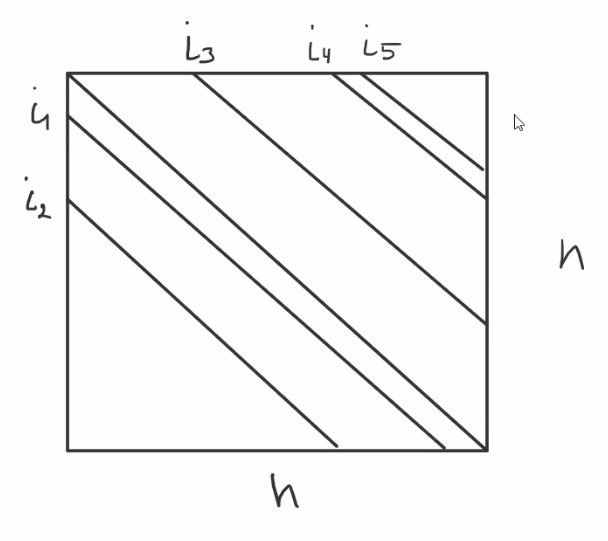
\includegraphics[scale=0.3]{10_1.png}
\end{center}
\begin{itemize}
\item \(n \times n\), где \(n\) --- размерноесть исходной матрицы, \(m\) --- количество ненулевых диагоналей
\end{itemize}
\subsection{Ленточный формат}
\label{sec:orgb1d0793}
\begin{center}
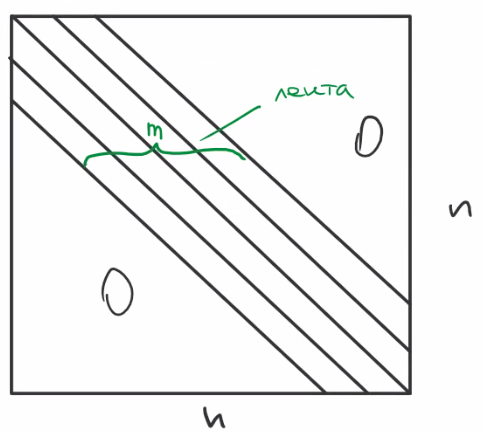
\includegraphics[scale=0.3]{10_2.png}
\end{center}
\(a_{ij} = 0\), если \(|i - j| > k\), \(k\) --- полуширина, \(m = 2k + 1\) --- ширина ленты
\subsection{Профильный формат}
\label{sec:org5bad7a8}
\begin{center}
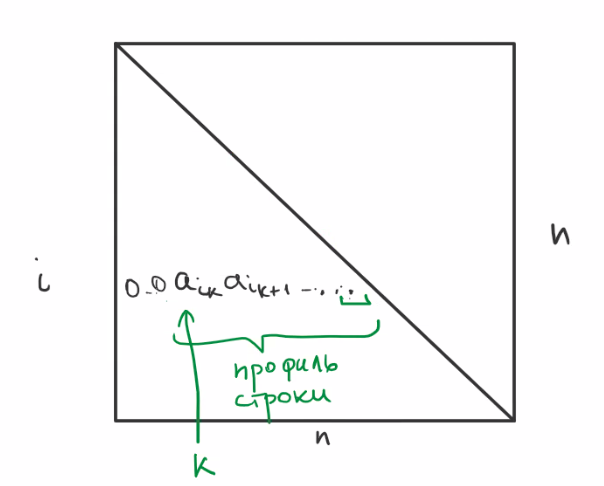
\includegraphics[scale=0.3]{10_3.png}
\end{center}
Обычно хранят несимметричный матрицы. Структуры хранения:
\begin{itemize}
\item Вещественный массив \(di[n]\) --- массив диагональных элементов
\item Вещественные массивы \(al\) --- элементы нижнего треугольника по строками, \(au\) --- эленметы верхнего треугольника по столбцам
\item Целочисленный массив \(ia(k) =\)индекс\color{red}(в нумерации с 1)\color{black}, с которого начинаются элементы \(k\)-ой строки(столбца) в массивах \(al,\ au\). Размерноть равна \(n + 1\), при чем \(ia[n + 1]\) равен индексу первого незанятого элемента в \(al,\ au\), \(a[n + 1] - 1\) --- размерность \(al\) и \(au\).
\end{itemize}
\begin{examp}
\-
\[ \begin{matrix}
a_{11} & & & & & & & & \\
0 & a_{22} & a_{23} & a_{24} & & &  \text{\huge0}& &  \\
0 & a_{32} & a_{33} & 0 & a_{35} & a_{36} & & &  \\
0 & a_{42} & 0 & a_{44} & a_{45} & 0 & a_{47} & &  \\
& & a_{53} & a_{54} & a_{55} & a_{56} & 0 & a_{58} & a_{59} \\
& & a_{63} & 0 & a_{65} & a_{66} & 0 & a_{68} & 0 \\
& & & a_{74} & 0 & 0 & a_{77} & 0 & a_{79} \\
& \text{\huge0}& &  & a_{85} & a_{86} & 0 & a_{88} & 0 \\
& & &  & a_{95} & 0 & a_{97} & 0 & a_{99}
\end{matrix} \]

\[ di = \{a_{11}, a_{22}, a_{33}, a_{44}, a_{55}, a_{66}, a_{77}, a_{88}, a_{99}\} \]
\[ ia = \{1, 1, 1, 2, 4, 6, 9, 12, 15, 19\} \]
\[ al = \{a_{32}, a_{42}, 0, a_{53}, a_{54}, a_{63}, 0, a_{65}, a_{74}, 0, 0, a_{85}, a_{86}, 0, a_{95}, 0, a_{97}, 0\} \]
\[ au = \{a_{23}, a_{24}, 0, a_{35}, a_{45}, a_{36}, 0, a_{56}, a_{47}, 0, 0, a_{58}, a_{68}, 0, a_{59}, 0, a_{79}, 0\} \]
Для 6й строки: \(al[ia[6]] = al[6] = a_{63}\), профиль 6й строки \(ia[7] - ia[6] = 9 - 6 = 3\)
\begin{enumerate}
\item \(al[6] = a_{63}\)
\item \(al[7] = 0\)
\end{enumerate}
\end{examp}
\chapter{}
\label{sec:orgbe50d6d}
\section{Разреженный формат}
\label{sec:org0b56101}
\subsection{Строчно столбцовый формат}
\label{sec:org799db20}
\begin{enumerate}
\item Вещественный массив \(di[n]\) --- диагональные элементы
\item Вещественный массив \(al, au\) --- по строкам и стобцам соответсвенно
\item Целочисленный массив \(ja\) --- содержит номера столбцов (строк)
хранимых внедиагональных элементов нижнего(верхнего) треугольника
матрицы. \(j \le m\), где \(m\) --- размерность массивов \(ja, al, au\), \(ja[j]\) --- номер столбца для \(al[j]\), или номер строки для \(au[j]\)
\item Целочисленный массив \(ia\), \(ia[k]\) --- равен индексу(в нумерации с 1) с которого начинается \(k\)-той строки(столбца)
\end{enumerate}
Размерность \(ja, al, au\): \(ia[n + 1] - 1\). \(ia[i + 1] - ia[i]\) --- количество хранимых внедиагональных элементов \(i\)-той строки(столбца) нижнего(верхнего) треугольника. \(ia\) и \(ja\) --- портрет матрицы.

\begin{examp}
\-
\[ \begin{matrix}
a_{11} & & & & & & & & \\
0 & a_{22} & a_{23} & a_{24} & & &  \text{\huge0}& &  \\
0 & a_{32} & a_{33} & 0 & a_{35} & a_{36} & & &  \\
0 & a_{42} & 0 & a_{44} & a_{45} & 0 & a_{47} & &  \\
& & a_{53} & a_{54} & a_{55} & a_{56} & 0 & a_{58} & a_{59} \\
& & a_{63} & 0 & a_{65} & a_{66} & 0 & a_{68} & 0 \\
& & & a_{74} & 0 & 0 & a_{77} & 0 & a_{79} \\
& \text{\huge0}& &  & a_{85} & a_{86} & 0 & a_{88} & 0 \\
& & &  & a_{95} & 0 & a_{97} & 0 & a_{99}
\end{matrix} \]

\[ di = [a_{11}, a_{22}, a_{33}, a_{44}, a_{55}, a_{66}, a_{77}, a_{88}, a_{99}] \]
\[ ia = [1, 1, 1, 2, 3, 5, 7, 8, 10, 12] \]
\[ ja = [2, 2, 3, 4, 3, 5, 4, 5, 6, 5, 7] \]
\[ al = [a_{32}, a_{42}, a_{53}, a_{54}, a_{63}, a_{65}, a_{74}, a_{85}, a_{86}, a_{95}, a_{97}] \]
\[ au = [a_{23}, a_{24}, a_{35}, a_{45}, a_{36}, a_{56}, a_{47}, a_{58}, a_{68}, a_{59}, a_{79}] \]
Для шестой строчки: \(ia[6] = 5\) --- начало шестой строчки в массиве \(ja\) и \(al\). \(ia[6 + 1] - ia[6] = 7 - 5 = 2\) --- количество элементов.
\begin{enumerate}
\item \(ja[ia[6]] = ja[5] = 3\)
\item \(ja[ia[6] + 1] = ja[6] = 5\)
\end{enumerate}
\end{examp}
\subsection{Решение СЛАУ. Метод Гаусса}
\label{sec:org97d20f7}
\[ \begin{cases}
a_{11}x_1 + a_{12} x_2 + \dots + a_{1n}x_n = b_1 \\
a_{21}x_1 + a_{22} x_2 + \dots + a_{2n}x_n = b_2 \\
\vdots \\
a_{n1}x_1 + a_{n2} x_2 + \dots + a_{nn}x_n = b_n
\end{cases} \]

\[ Ax = b \]
\begin{itemize}
\item \(A = (a_{ij})_{i,j = 1}^n\) --- вещественные числа
\item \(b = (b_1, b_2, \dots, b_n)^T\)
\item \(x = (x_1, x_2, \dots, x_n)^T\)
\end{itemize}
\(-\frac{a_{21}}{a_{11}}, -\frac{a_{31}}{a_{11}}, \dots, -\frac{a_{n1}}{a_{11}}\)
Верхний индекс обозначает этап.
\[ \begin{cases}
a_{11}x_1 + a_{12} x_2 + \dots + a_{1n}x_n = b_1 \\
a_{22}^{(1)}x_2 + a_{23}^{(1)}x_3 + \dots + a_{2n}^{(1)}x_n = b_2^{(1)} \\
a_{32}^{(1)}x_2 + a_{33}^{(1)}x_3 + \dots + a_{3n}^{(1)}x_n = b_3^{(1)} \\
\vdots \\
a_{n2}^{(1)}x_2 + a_{n3}^{(1)}x_3 + \dots + a_{nn}^{(1)}x_n = b_n^{(1)}
\end{cases} \]
\[ a_{ij}^{(1)} = a_{ij} - \frac{a_{i1}}{a_{11}}a_{1j} \quad b_i^{(1)} = b_i - \frac{a_{i1}}{a_{11}}b_1 \quad i,j = \overline{2, n}\]
\begin{remark}
\(a_{11} \neq 0\)
\end{remark}

\[ \begin{cases}
a_{11}x_1 + a_{12} x_2 + \dots + a_{1n}x_n = b_1 \\
a_{22}^{(1)}x_2 + a_{23}^{(1)}x_3 + \dots + a_{2n}^{(1)}x_n = b_2^{(1)} \\
a_{33}^{(2)}x_3 + a_{34}^{(2)}x_4 + \dots + a_{3n}^{(2)}x_n = b_3^{(2)} \\
\vdots \\
a_{n3}^{(2)}x_3 + a_{n4}^{(2)}x_4 + \dots + a_{nn}^{(2)}x_n = b_n^{(2)}
\end{cases} \]
\[ a_{ij}^{(2)} = a_{ij}^{(1)} - \frac{a_{i2}^{(1)}}{a_{22}^{(1)}}a_{2j}^{(1)} \quad b_i^{(2)} = b_i^{(1)} - \frac{a_{i2}^{(1)}}{a_{22}^{(1)}}b_2^{(1)} \]

\(n - 1\) этап:

\[ \begin{cases}
a_{11}x_1 + a_{12} x_2 + \dots + a_{1n}x_n = b_1 \\
a_{22}^{(1)}x_2 + a_{23}^{(1)}x_3 + \dots + a_{2n}^{(1)}x_n = b_2^{(1)} \\
a_{33}^{(2)}x_3 + a_{34}^{(2)}x_4 + \dots + a_{3n}^{(2)}x_n = b_3^{(2)} \\
\vdots \\
a_{nn}^{(n - 1)}x_n = b_n^{(n - 1)}
\end{cases} \]

\[ a_{ij}^{(k)} = a_{ij}^{(k - 1)} - \frac{a_{ik}^{(k - 1)}}{a_{kk}^{(k - 1)}}a_{kj}^{(k - 1)} \quad b_i^{(k)} = b_i^{(k - 1)} - \frac{a_{ik}^{(k - 1)}}{a_{kk}^{(k - 1)}}b_k^{(k - 1)} \quad \ k \in \overline{1, n};\ i,j \in \overline{k + 1, n}\]
\subsection{Обратный ход Гаусса}
\label{sec:org8f797c2}
\[ x_n = \frac{b_n^{(n - 1)}}{a_{nn}^{(n - 1)}} \]
\[ \vdots \]
\[ x_2 = \frac{b_2^{(1)} - a_{23}^{(1)} x_3 - \dots - a_{2n}^{(1)}x_n}{a_{22}^{(1)}} \]
\[ x_1 = \frac{b_1 - a_{12} x_2 - \dots - a_{1n} x_n}{a_{11}} \]
\[ x_k = \frac{b_k^{(k - 1)} - \sum_{i = k + 1}^n a_{ki}^{(k - 1)} x_i}{a_{kk}^{(k - 1)}} \quad k \in \overline{n, 1}\]
\(\sum_j^n = 0\), если \(j > n\)
\begin{rualgo}[H]
\caption{метод Гаусса}
\begin{algorithmic}[1]
\FOR{\(k = 1,\dots, n - 1\)}
  \FOR{\(i = k+1,\dots,n\)}
    \STATE \(t_{ik} = \frac{a_{ik}}{a_{kk}}\)
    \STATE \(b_i = b_i - t_{ik}b_k\)
    \FOR{\(j = k + 1,\dots,n\)}
      \STATE \(a_{ij} = a_{ij} - t_{ik}a_{kj}\)
    \ENDFOR
  \ENDFOR
\ENDFOR
\STATE \(x_n = \frac{b_n}{a_{nn}}\)
\FOR{\(k = n - 1,\dots, 1\)}
  \STATE \(x_k = \frac{(b_k - \sum_{j = k + 1}^n a_{kj} x_j)}{a_{kk}}\)
\ENDFOR
\end{algorithmic}
\end{rualgo}

Модификация с постолбцовым выбором глваного элемента
\begin{rualgo}[H]
\caption{Модификация алгоритма Гаусса}
\begin{algorithmic}[1]
\STATE \(m:\ m \ge k,\ |a_{mk}| = \max_{i \ge k}\{|a_{ik}|\}\)
\IF{\(a_{mk} = 0\)}
\STATE Нет однозначного решения. Завершить алгоритм
\ELSE
\FOR{\(j = k,\dots,n\)}
\STATE Поменять местами \(b_x\) и \(b_m\)
\STATE Поменять местами \(a_{kj}\) и \(a_{mj}\)
\ENDFOR
\ENDIF
\end{algorithmic}
\end{rualgo}
\end{document}
